\documentclass{article}
\usepackage{graphicx}
\usepackage[margin=1.5cm]{geometry}
\usepackage{amsmath}

\begin{document}

\title{Monday Reading Assessment: Unit 2, Terminal Voltage}
\author{Prof. Jordan C. Hanson}

\maketitle

\section{Memory Bank}

\begin{itemize}
\item $V = i R$ ... Ohm's Law, with $V$ for voltage, $i$ for current, and $R$ for resistance.
\item $R_{tot} = R_1 + R_2$ ... Total resistance of two resistors in series.
\end{itemize}

\section{Batteries and Internal Resistance}

\begin{enumerate}
\item Did you know that batteries have resistance?  Consider Fig. \ref{fig:1}, in which the resistance $r$ of a battery is shown, in series with a resistor $R$.  The AA battery \textit{is supposed to have 1.5 V}, but it also has an internal resistance of $r = 1\Omega$.  Think of $\epsilon$ as the ideal 1.5 V of the AA battery.  (a) If $R = 50\Omega$, what is the current flowing from the battery?  You can think of $r$ and $R$ as \textbf{in series.}  (b) The battery terminal voltage is $V = \epsilon - Ir$, and $\epsilon$ is always 1.5 V.  If $I$ is the current, what is $V$? (c) What power is consumed in this circuit, and what fraction is consumed by the battery?
\end{enumerate}

\begin{figure}
\centering
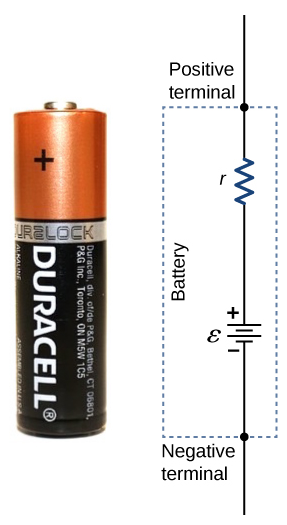
\includegraphics[width=0.17\textwidth]{duracell.png} \hspace{3cm}
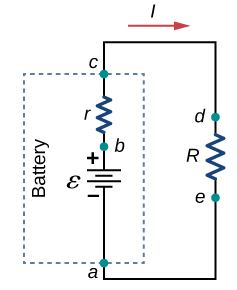
\includegraphics[width=0.25\textwidth]{duracell2.png}
\caption{\label{fig:1}(Left) The AA battery has a voltage $\epsilon$ and a resistance $r$, in series.  (Right) Connecting the model battery to a resistance $R$ in series.}
\end{figure}

\end{document}
